%Erzeugt mit dem LaTeX-Generator: http://latex.sehnot.de

%Schriftgröße, Layout, Papierformat, Art des Dokumentes
\documentclass[12pt,oneside,a4paper]{scrbook}

%Einstellungen der Seitenränder
\usepackage[left=3cm,right=2cm,top=2cm,bottom=2cm,includeheadfoot]{geometry}

%neue Rechtschreibung
%\usepackage[ngerman]{babel}

%Umlaute ermöglichen
% \usepackage{fontspec}
% \setromanfont{TeX Gyre Pagella}

% \usepackage[math-style=iso]{unicode-math}
% \setmathfont{Asana Math}

\usepackage{graphicx}
\usepackage{wrapfig}
\usepackage[utf8x]{inputenc}
\usepackage{url}
\usepackage{multirow}
\usepackage{amsmath}
\usepackage{hyperref}
\usepackage{multicol}
\usepackage{amsthm}
\usepackage[official]{eurosym}
\usepackage{setspace}
%Zitieren
\usepackage[longnamesfirst, authoryear]{natbib}
\usepackage{minted}
\usepackage{booktabs}



%Kopf- und Fußzeile
\usepackage{fancyhdr}
\pagestyle{fancy}
\fancyhf{}

\newcommand{\HRule}{\rule{\linewidth}{0.5mm}}

%Kopfzeile rechts bzw. außen
\fancyhead[R]{\nouppercase{\leftmark}}
%Linie oben
\renewcommand{\headrulewidth}{0.5pt}

%Fußzeile links bzw. innen
\fancyfoot[L]{Units of Measure - a Scala Macro System}
%Fußzeile rechts bzw. außen
\fancyfoot[R]{\thepage}
%Linie unten
\renewcommand{\footrulewidth}{0.5pt}

\clubpenalty = 50000
\widowpenalty = 50000




\title{Units of Measure - a Scala Macro System}
\author{Julian Schrittwieser}
\date{\today}

\begin{document}


\begin{titlepage}

\begin{center}


% Upper part of the page

\includegraphics[width=0.4\textwidth]{tu-logo.png}\\[3cm]


\textsc{\Large Software \& Information Engineering}\\[0.5cm]


% Title
\HRule \\[0.8cm]
{ \huge \bfseries Units of Measure}\\[0.4cm]
\Large A Scala Macro System

\HRule \\[1.5cm]

\vfill


% Author and supervisor
\begin{minipage}{0.4\textwidth}
\begin{flushleft} \large
\emph{Author:}\\
Julian \textsc{Schrittwieser}
\end{flushleft}
\end{minipage}
\begin{minipage}{0.4\textwidth}
\begin{flushright} \large
\emph{Advisor:} \\
Univ.-Prof. Dr. Jens \textsc{Knoop}
\end{flushright}
\end{minipage}

\vfill

% Bottom of the page
{\large Februar 12th, 2013}

\end{center}

\end{titlepage}

\pagenumbering{roman} % Roman numerals, other styles possible: http://www.image.ufl.edu/help/latex/intext.shtml
\setcounter{page}{2}

% \onehalfspacing
\chapter*{Preface}

This thesis completes my Bachelor in Software \& Information Engineering at the Vienna University of Technology. It was written at the Complang Group, part of the Institute of Computer Languages of the Faculty of Informatics.

It was a pleasure to work on such an interesting problem with a vibrant language like Scala - I would like to thank Prof. Dr. Jens Knoop for making this possible, as well as for advising me about the scope and direction of this work. He also provided invaluable feedback and advice, helping to make this thesis what it is now.

I would also like to express my special thanks to Eugene Burmako, creator and maintainer of the Scala Macro system. Without his work, this Units of Measure system would not have possible - both because it builds on his macros and because he provided essential help in their use.

Finally, a big thank you to the Scala community in general, especially the \verb|#scala| IRC channel on Freenode and the Scala mailing list.
\\ \\
Vienna, May 17th, 2013  \hfill Julian Schrittwieser

\singlespacing
\tableofcontents
%\onehalfspacing

\chapter{Introduction}
\pagenumbering{arabic} % Roman numerals
\setcounter{page}{1}

Units of Measurement are fundamental to many endeavors, often so important that their usage and definition is mandated by law. Today, the International System of Units (SI) is in wide use, along with legacy systems like the Imperial system. These coexisting unit systems are also a source of confusion and accidents - in September 1999, NASA lost the Mars Climate Orbiter due to a mix-up between Newton and pound force \citep{Nasa99}. Even earlier, a Boeing 767 ran out of fuel in mid-flight, again because of mistakes related to Imperial and Metric unit systems \citep{Witkin83}.


\section{Motivation}

Almost as long as high-level programming languages have existed, there have been attempts to enhance them with proper Units of Measure systems. A very early paper from Narain Gehani extends quantities in Pascal and Fortran with a special \emph{UNITS} attribute to be able to detect errors missed by the normal type system \citep{Gehani1977}. The approaches vary wildly: Allen et al. present an object oriented Units of Measure system based on statically typed metaclasses \citep{Allen04}.  More recently, Hills et al. introduce a static analyzer for the C programming language, based solely on annotations in source comments \citep{Hills2012}.

As of the writing of this paper, there is no comprehensive Units of Measure system for the Scala programming language. Additionally, the introduction of compile time macros in the most recent version of the language (2.10) offers an unique opportunity: For the first time, it is possible to create a solely type-based unit system that is not restricted to predefined base units, but can be extended arbitrarily.

\section{Structure}

In this paper, I first give an overview of Units of Measure systems currently in use in other languages. I then go on to describe my own implementation in detail, starting with the objectives I'm trying to achieve and the limitations my system has. Next, details of the implementation are given, before usage examples are shown. Finally, benchmarks are used to verify the objectives from the beginning and an outlook into future work concludes the paper.


\section{Nomenclature}
Throughout this paper, I use \emph{Measure} to refer to a number annotated with its corresponding units. The exact implementation of this annotation depends on the context, some libraries use static type informations, others fields in an object. \emph{Units of Measure} is used to refer to any system that provides such an implementation, including methods to perform arithmetic with \emph{Measure}s. \emph{Units} are the physical units in abbreviated or full form that the Measure is used to represent. Examples include \verb|m/s| for speed or \verb|kg*m/s^2 == N| for force.

\section{Source Code}
The source code for all benchmarks mentioned can be found on GitHub: \url{https://github.com/Mononofu/Units-of-Measure/tree/master/thesis/benchmarks}. This same repository also contains the source for this document (\url{https://github.com/Mononofu/Units-of-Measure/tree/master/thesis}) as well as the implementation of the Units of Measurement system in Scala (\url{https://github.com/Mononofu/Units-of-Measure}). All code is provided under the GNU General Public License, version 3, as is and without warranty of any kind.

\section{Code Organization}

% TODO: describe repo layout here



\chapter{Related Work}

In principle, there are two distinct ways to implement units of measurement in a programming language: Either statically as part of the type system, or dynamically with objects that know their own unit. Each approach has its own merits and disadvantages, so in the following I examine a few existing implementations in common languages before creating my own solution.

\section{Dynamic Systems}

Some programming languages do not give their users much choice, because they either completely lack static type systems (dynamic languages like Python or Ruby) or their type system is not sophisticated enough for a units of measurement library. In general, those dynamic systems allow access to unit information at runtime but in turn pay a heavy performance price: Each number is stored as a full blown object (see figure \ref{code:naive_java_measure}), not as a simple primitive like a normal number. Thus, all calculations incur additional memory lookups and values take additional space.

\begin{figure}
\begin{minted}{java}
class Measure<T extends java.lang.Number> {
  T      value;
  Unit   unit;
}
\end{minted}
\caption{A naive implementation of a number annotated with its unit in Java. Actual size depends on the number used, but at least 8 bytes are used by the object itself, and further 4/8 bytes (32/64 bit system, resp.) are needed for the reference to the unit.}
\label{code:naive_java_measure}
\end{figure}



\subsection{Java - JScience}

Java has a standardized Units of Measurement API \citep{Units13} with several implementations, both open source and commercial. I will focus on JScience here \citep{Dautelle11}. In addition to support for physical units, JScience also contains libraries for simple mathematical functions, currencies and a linear algebra module. Here, I only focus on parts pertaining to Units of Measurement.

JScience represents Measures using the class \verb/Amount/, but users are free to create their own implementations of \verb/Measurable/. Measures are created with a flexible static helper function (\verb/valueOf/) from a range of different inputs. For details, see the short usage example below in Figure \ref{code:jscience_example}. Essentially, \verb/Amount/ is a wrapper class that tags a number with its corresponding unit - as shown in \ref{code:naive_java_measure} - and provides a set of helper and conversion functions.

\begin{figure}
\begin{minted}{java}
Amount<Mass> m0            = Amount.valueOf(100, POUND);
Amount<ElectricCurrent> m1 = Amount.valueOf("234 mA").to(MICRO(AMPERE));

// m0 =    100 lb
// m1 = 234000 uA

Unit<Mass> u  = m0.getUnit();
Dimension d   = u.getDimension();

\end{minted}
\caption{Example for JScience from the official documentation \citep{Dautelle11}. Usage is straightforward and unit information is still available at runtime.}
\label{code:jscience_example}
\end{figure}

Unit safety is enforced both by the type system at compile time (Measures are generic classes with their units as type parameters) and comparison functions at run time (\verb/equals/ only returns true if both the value and the interval match, etc.).

Unfortunately, the performance hit due to the wrapper classes is quite severe - I experienced a slowdown of around 80 on my machine in a simple benchmark, compared to normal primitives (\verb/int/ and \verb/double/) (see Figure \ref{bench:jscience}).

At the moment, Units of Measurement Systems in Java are only practicable in systems that are not performance critical. Alas, many systems that would benefit most are performance critical - computer game engines, high frequency trading, etc. Therefore, Units of Measurements remain a niche application in Java.

\begin{figure}
\begin{tabular}{lrrr}
method          & int    & double  & JScience \\
\midrule
addition        & 1.0 ns &  1.8 ns    &   149.5 ns \\
multiplication  & 1.1 ns &  1.9 ns    &   162.3 ns
\end{tabular}
\caption{A simple benchmark of JScience compared to primitives data types. JScience is at least 80 times slower on average.}
\label{bench:jscience}
\end{figure}


\subsection{Python - units}

Python is a dynamic language, so the only way to make a system of measurements work is to create a dynamic system that relies on tagged numbers. That's exactly what \emph{units} \citep{Donohue12} does. Usage is very simple, as seen in Figure \ref{code:python_units}. Thanks to operator overloading and the dynamic nature of Python code, units can be introduced into legacy code with only a few changes.

\begin{figure}
\begin{minted}{python}
metre, second = unit('m'), unit('s')                   # define units
print(metre(10) / second(2))                           # 5 m / s
newton = named_unit('N', ['kg', 'm'], ['s', 's'], 1)   # 1 N = 1 kg*m/s^2
units.predefined.define_units()                        # SI units and more
\end{minted}
\caption{\emph{units} makes it very simple to define custom units and to add conversions to existing units, while also including all standard units for immediate use. Calculation happens just like with primitives, thanks to operator overloading.}
\label{code:python_units}
\end{figure}



\begin{figure}
\begin{tabular}{lrrr}
method          & int    & double  & units \\
\midrule
addition        & 151 ns &  164 ns    &    4.136 ns \\
multiplication  & 159 ns &  165 ns    &   22.352 ns
\end{tabular}
\caption{Even though Python is an interpreted language, there is a large difference between primitive numbers, and those provided by the \emph{units} library. The slowdown is especially severe for the multiplication as a new unit has to be generated for the result.}
\label{bench:python_units}
\end{figure}


\section{Static Systems}

Static systems are the complete opposite compared to dynamic systems: They usually do not provide any unit information at runtime, but also do not incur any performance overhead - all units are checked at compile time. To achieve this, they rely on a powerful type system or even compiler plugins, effectively offloading much of the work on the compiler.

\subsection{F\#}

\verb/F#/ is one of only a few languages that have integrated a system of units into the language itself. This allows for easy usage and definition of units since they can rely on special syntax.
\citep{Kennedy08:1}

As usual, \verb/F#/ comes with all common units - both SI and Imperial - predefined \citep{Kennedy08:2}, but it's also easy to interface with code that is not unit aware: Primitive types like \verb/float/ are just a type alias for \verb/float<1>/ (a float with unit dimension).

Thanks to the language support, units also work with generics, including full type (unit) inference. As an example, if we define a simple function \verb/let sqr(x: float<_>) = x*x/, \verb/F#/ will automatically infer that it takes any \verb/float<'u>/ and returns a \verb/float<'u^2>/ \citep{Kennedy08:3}. This works for types of arbitrary complexity, making the programmers life much simpler.

The support for generics also extends to custom types - it's enough to annotate a type parameter with \verb/[<Measure>]/ to make it a unit parameter \citep{Kennedy08:4}. For a example, see Figure \ref{code:fsharp}.


\begin{figure}
\begin{minted}{fsharp}
[<Measure>] type kg                 // define a unit
let gravity = 9.81<m/s^2>           // use units
// generic type
type Vector2< [<Measure>] 'u > = { x: float<'u>, y: float<'u> }
\end{minted}
\caption{Usage examples for the unit system in F\#.}
\label{code:fsharp}
\end{figure}

\subsection{C++ - Boost.Units}

The \verb/Boost.Unit/ library takes advantage of the power of C++ templates in the form of the Boost Metaprogramming Library (MPL).  It relies on the compiler to adequately optimize the code, but then incurs no performance overhead at runtime \citep{Schabel10}.However, since it heavily relies on template metaprogramming it has stringent requirements for the compiler and only works on new, standard compliant compilers.

Variable definitions work as always (\verb/quantity<length> L = 2.0*meters;/), and thanks to operator overloading arithmetic is exactly the same as for primitives.

\verb/Boost.Unit/ is also independent of any single unit systems - functions can be defined generically, for arbitrary unit systems, using just the types of the dimensions. For an example, see Figure \ref{code:boost_units_generic}. Users can then define their own unit systems to interface with already existing library code.

\begin{figure}
\begin{minted}{c++}
template<class System,class Y>
quantity<unit<energy_dimension,System>,Y>
work(quantity<unit<force_dimension,System>,Y> F,
     quantity<unit<length_dimension,System>,Y> dx)
{
    return F*dx;
}
\end{minted}
\caption{The physical definition of work - computed for an arbitrary unit system, from \citep{Schabel10}.}
\label{code:boost_units_generic}
\end{figure}


\subsection{Haskell - Dimensional}
Haskell's \verb/Dimensional/ module \citep{Buckwalter06} completely relies on the type system and is the most elegant of the unit systems presented here. It relies on a single data type (\verb/Dimensional/, see Figure \ref{code:haskell_dimensional}), parameterized with the exponents of different physical dimensions (Figure \ref{code:haskell_dim}). While only integer exponents are possible, rational exponents can be avoided in practice.

\begin{figure}
\begin{minted}{haskell}
newtype (Variant v, Dims d)
      => Dimensional v d a = Dimensional a deriving (Show, Eq, Ord)
\end{minted}
\caption{Dimensional, the unit system's fundamental data type. Since 'a', representing the underlying number, is the only non-phantom type Dimensional is defined as a newtype and does not incur any runtime overhead. From \citep{Buckwalter06}.}
\label{code:haskell_dimensional}
\end{figure}



\begin{figure}
\begin{minted}{haskell}
data (NumType l,    -- Length.
      NumType m,    -- Mass.
      NumType t,    -- Time.
      NumType i,    -- Electric current.
      NumType th,   -- Thermodynamic temperature.
      NumType n,    -- Amount of substance.
      NumType j)    -- Luminous intensity.
   => Dim l m t i th n j

type DLength      = Dim Pos1 Zero Zero Zero Zero Zero Zero
type DForce       = Dim Pos1 Pos1 Neg2 Zero Zero Zero Zero
\end{minted}
\caption{The type Dim, containing the physical base dimensions, and two derived dimesions, from \citep{Buckwalter06}.}
\label{code:haskell_dim}
\end{figure}


As with the other systems, operator overloading allows for easy calculations. \verb/*~/ and \verb|/~| can be used to attach units to numbers and remove them again.


\begin{figure}
\begin{minted}{haskell}
escapeVelocity :: (Floating a) => Mass a -> Length a -> Velocity a
escapeVelocity m r = sqrt (two * g * m / r)
  where
    two = 2 *~ one
    g = 6.6720e-11 *~ (newton * meter ^ pos2 / kilo gram ^ pos2)
\end{minted}
\caption{An example function using the Dimensional module, from \citep{Buckwalter06}.}
\label{code:haskell_dimensional}
\end{figure}

\verb/Dimensional/ is restricted to the physical dimensions mentioned in Figure \ref{code:haskell_dim}. To add more dimensions, the fundamental data type would have to be changed - unfeasible in practice.


\subsection{Scala}

Scala also has a long history of attempts to introduce Units of Measure. One of the oldest of such attempts is a now defunct compiler plugin \citep{Nygard09}. It allowed the programmer to introduce units using multiplication (\verb/400.0*m*m/) and caught common errors when combining units in invalid ways. Sadly, it's only compatible with Scala up to version 2.7.1 - as of 2013, the most recent version is 2.10.0.

Another such example comes from \citep{McBeath08}, who implements a simple unit system based on Church Numerals. However, just as Haskell's \verb/Dimensional/ it is restricted to predefined units and does not allow the user to define her own units.

Finally, there is \verb/ScalaQuantity/ \citep{Hans12}, which is closely modeled on Haskell's \verb/Dimensional/. Again, it does not allow user defined units and is otherwise so similar to \verb/Dimensional/ that I won't cover it in detail.

Currently, there is no Units of Measure system in Scala that allows user defined units or provides for calculations without runtime overhead. This inspired me to create my own library, which I cover in the following.

\chapter{Objectives}

As we have seen, there are a few common features that almost all systems support (custom units, conversions), while some aspects are limited to more advanced libraries (generics, no runtime overhead). I aim to make my Units of Measure system as comprehensive as possible, therefore I present a short summary of all desirable features here. This summary serves as a reference for my implementation, as well as a handy reminder for the reader.


\begin{description}
  \item[No Runtime Overhead] This is one of the most important goals - in many systems that profit from unit checking (games, embedded systems), computing power is at a premium during runtime, while processing at compile time is of little consequence. This also extends to memory consumption - Measures should need no more space than primitive numbers. In fact, they should be indistinguishable at runtime.

  \item[Static Unit Checking] Any mistakes in the units of variables should be detected at compile time - there should not be any surprises at runtime! This is also closely related to the goal above. In fact, it is only possible to check units at compile time, as there is no unit information left at runtime. A simple way to achieve this - also the own I intend to use - is to offload the work of enforcing unit correctness onto the type system, by for example specifying the units as type parameters.

  \item[Custom Units] While it is imperative to provide a thorough selection of units - the SI system at the very least -, it is simply impossible to collect and implement every possible unit. One Application might make heavy use from different types of currency, while another is solely concerned with physical temperatures. Therefore it should be possible for the user to define his own units, as well as to connect them to already existing units so that automatic conversion can take place.

  \item[Unit Conversion] To take full advantage of the provided units, helper methods should automatically convert numbers between different unit systems, as specified by the user. For example, \verb|u(10, "m/s").as("km/h")| automatically changes the units of the Measure and adjusts its value accordingly, to \verb/36/. Naturally, this relationship between units needs to be reflected in their definition, otherwise automatic conversions are impossible.

  \item[Access to a Measure's Units] While it is impossible to access unit information at runtime - see the first goal -, it should still be possible to query the unit of a Measure when its type is known. This is essentially a way to pretty print the underlying type information for a human reader.

  \item[Generics] Another very important aspect is the support of generic classes and methods. A clarifying example: \verb|def square[T](n: T) = n*n| should automatically infer that its return type is T with all units squared. The same principle extends to classes, the most common use case being a simple vector of numbers that defines operations like addition or dot product.

  \item[Implementations for common primitives, as well as all instances of Numeric] Finally, it should be possible to use every type that is an instance of Numeric (that is, every type that can be used as a number) as the underlying type for a Measure. Additionally, special support should be provided for primitives (int, long, float, double), since their performance is the most critical.

\end{description}

\section{Limitations}
\label{sec:limitiations}

Before I describe my implementation in detail, I provide a short list of its limitations. Those are mostly based on limitations of the JVM itself, or on more fundamental issues.

\begin{description}
  \item[Measure is not an instance of Numeric] While Measure requires its underlying type to be an instance of Numeric, it cannot be such an instance itself. The reason is simple: Multiplication will result in a Measure with a different type than the two operands (the units change), thus violating the type bounds of Numeric. The same can even happen for simple addition: Since all operations with a Measure canonicalize (reduce and sort) its type argument (representing its unit), it is possible that an addition of two Measures results in a Measure with a different type.

  \item[Runtime equality ignores units] Since one fundamental goal was to incur no runtime overhead, it is obviously impossible to check unit equality at runtime. In fact, due to the nature of my implementation, Measures based on primitives are indistinguishable from those primitives at runtime - the wrapping Measure class only exists during compilation.

  \item[Generics require Macros] In Java and all languages based on it, generics are implemented in a simple way: The type parameter is only known to the compiler, at runtime the generic class is represented by its raw counterpart. Therefore, all type parameters share the same single method/class - unlike C++, where a separate instance of the generic class is generated for each and every different type parameter. This presents a problem for the Measure macros, since they need to know the Measure's actual type parameter to correctly perform their work (In normal Scala code, it is only known that there is some \verb|Measure[T]|, not very helpful).

  The solution to this problem is to define all generic methods that use Measures as macros, essentially mirroring the way C++ templates are implemented in Scala. As a downside, the Measure macros will be called every time the generic method is used, not just once for each type parameter.

  \item[Arrays lead to degraded Performance] Due to choices made in the current implementation of value classes in Scala, and issues with arrays on the JVM, Measures experience degraded performance when placed in arrays. While the Measure wrapper class is normally only present at compile time for primitives, arrays force the Measure class to stay present - essentially requiring an explicit boxing/unboxing step for each calculation done with the Measure, and also resulting in an increased memory usage. As a workaround, Vector classes with explicit members can be used to reduce the memory overhead.


\end{description}

\chapter{Implementation}

The implementation of my Units of Measure system rests on a few cornerstones that I present here. Without those, this system would not be possible, at least not without sacrificing a few of its goals. Some of those features (like Type Macros) are still very experimental and only available in nightly builds of Scala 2.11. Therefore, my library does not work with the current stable version of Scala (2.10 at the of writing). Luckily, it is very easy to use Scala 2.11 even now - builds are provided over a Sonatype repository and can be used with a simple sbt include (sbt is the de facto standard build system for Scala).

\section{Design Principles}

First of all, for a Units of Measure system it is necessary to store the unit information for each number somehow. The easiest and most natural way is to turn the number into an object and include the unit information as a field, but this incurs additional overhead. To avoid this, I store unit information in type parameters - they don't need any space at runtime, since on the JVM they are eliminated by erasure. Unit expressions are represented as a simple linked list, a single node consists of a primitive unit and its exponent.

However, normally operations on those type parameters are cumbersome and make it difficult to use and implement a full unit system. Fortunately, with the introduction of macros in Scala 2.10, it is possible to perform arbitrary transformations on type parameters, and source code in general. For details on how macros work in Scala, see Section \ref{sec:macros}.

There is still one last problem: Arithmetic performance on boxed types is abysmal, and raw primitives can't have type arguments. Again, Scala 2.10 introduces a solution to this problem: Value classes. \ref{sec:value_classes}

To wrap up, you can see a full example of a Measure in Figure \ref{code:scala_measure}. As an additional optimization, I created separate implementations for the primitive types \verb|int|, \verb|long|, \verb|float| and \verb|double| in addition to the generic implementation for all types that are instances of \verb|Numeric|.

\begin{figure}
\begin{minted}{scala}
val u = new MeasureInt[CUnit[SUnit[Meter,  Pos1],
                             SUnit[Second, Neg2]]](10)
\end{minted}
\caption{A Measure representing the value $10 m/s^2$, with underlying type int.}
\label{code:scala_measure}
\end{figure}


\section{Macros in Scala}
\label{sec:macros}

Macros are what make a lot of the features of my Units of Measure system even possible in the first place. Fundamentally, macros in Scala are nothing more than normal functions that are executed by the compiler. Any arguments will be passed as abstract syntax trees (AST), and the result of the macro (another AST) is used in place of the original macro call. Those ASTs are the same data structures used by the compiler internally, and access to more specific APIs is possible using a special \verb|Context| object. I will cover the most relevant features here, for a full documentation please refer to \citep{Eugene13}.

For an example of a simple macro see Figure \ref{code:scala_macro} - macros in Scala don't use any special syntax, expect for the \verb|macro| keyword that tells the compiler that the current function is really a macro.



\begin{figure}
\begin{minted}{scala}
/* macro stub */
def u(nEx: Int, unitEx: String) = macro u_int_impl

/* macro implementation */
def u_int_impl(c: Context)
      (nEx: c.Expr[Int], unitEx: c.Expr[String]): c.Expr[Any] = {
  import c.universe._
  val comp = new Precomputer[c.type](c)
  val nID = comp.compute(nEx.tree)
  val parsedUnit = compute_unit(c)(unitEx)
  c.Expr(Block(comp.evals.toList, q"new MeasureInt[$parsedUnit]($nID)"))
}
\end{minted}
\caption{Scala macros always consist of two parts: The macro implementation itself - a scala function that takes AST expressions as arguments and returns a new AST - and the macro stub that references the actual implementation with the special macro keyword.}
\label{code:scala_macro}
\end{figure}


\subsection{Context and the Universe}

As mentioned above, the compiler API is exposed to the programmer using a special object, \verb|scala.reflect.macros.Context|, that every macro needs to accept as a parameter. As an example, the \verb|c: Context| object can be used to introduce new top-level classes (\verb|c.introduceTopLevel(packageName, classTree)|), raise compiler errors (\verb|c.abort(c.enclosingPosition, "error here")|) or search for already existing classes (\verb|c.mirror.staticClass(className)|). I use this API heavily to introduce new classes to store bookkeeping information about units, as well as to provide concise messages in case of errors.

Additionally, this includes the reflection API as a subpart, accessible via \verb|c.universe|. This API makes building (case classes) and deconstructing (via pattern matching) ASTs very easy.

\subsection{Type Macros}

Often, simple macro functions are not enough, especially to use macros in unorthodox positions. In my case, a helper macro for type definitions is necessary to make use of my library viable. In practice, type macros are very similar to normal macros - there are only two major differences: The macro stub is declared as a new type with \verb|type| instead of a new function with \verb|def|, and it returns a \verb|c.Tree| instead of a \verb|c.Expr|. For a short sample taken from my project see Figure \ref{code:scala_macro}.

Such type macros can be used anywhere a normal type can be used and can perform arbitrary calculations (including reading database schemata from disk or a remote server!).

\begin{figure}
\begin{minted}{scala}
/* macro stub */
type u_i(unitEx: String) = macro u_unit_int_impl

/* macro implementation */
def u_unit_int_impl(c: Context)(unitEx: c.Expr[String]): c.Tree = {
  val parsedUnit = compute_unit(c)(unitEx)
  import c.universe._
  AppliedTypeTree( Ident( TypeName("MeasureInt")), List( parsedUnit ) )
}
\end{minted}
\caption{Example of a type macro. Note that it is very similar to a normal macro, but returns a Tree instead of an Expression.}
\label{code:scala_typemacro}
\end{figure}

\subsection{Quasiquotes}

Construction of ASTs by hand is often very cumbersome. Luckily, there is a solution in the form of quasiquotes. They allow the user to write ASTs with normal Scala syntax, without knowing the internal data types used by the compiler. They also support substitution with \verb|$|, allowing for very concise Tree creation:

\verb|q"@macroimpl.LongName(n = $longName) class $classNameShort"|



\section{Value Classes}
\label{sec:value_classes}

On the Java Virtual Machine (JVM), optimal arithmetic performance is only possible with primitive data types. The downside is that they can't store any additional information, not even at compile time, since they don't accept type parameters.
Scala's value classes offer a solution to this problem. Value classes are a compile time wrapper around other types - similar to Haskell's \verb|newtype|. They also share the same limitations - a value class can only have a single field, type information is not available at runtime, etc.

Luckily, that's all that's needed for a Units of Measure system - unit information is available at compile time in the form of type parameters, and at runtime, performance is equal to normal primitives.


\section{Parser Combinators}

Parser Combinators make it very easy to write parsers for custom Domain Specific Languages (DSLs). For the Units of Measure library it was necessary to parse unit expressions similar to \verb|m / s^2|, as well as some internal parsing of type parameters. As their name implies, parser combinators are build from parsers (constant strings, regular expressions) that are combined with special combinators: repetition and alternatives. \citep{Spiewak09}

Such a parser is very close to the EBNF of the grammar it's supposed to parsed, allowing for an intuitive understanding of its purpose. For a short sample, see Figure \ref{code:scala_parse}

\begin{figure}
\begin{minted}{scala}
lazy val term: PackratParser[List[GeneralUnit]] =
  longFactor~rep(("*"|"/"|"")~longFactor) ^^ {
    case t~Nil => t
    case t~l => t ++ toTypenames(l) }
lazy val longFactor: PackratParser[List[GeneralUnit]] = (
    shortFactor~"^"~wholeNumber ^^ { case t~"^"~n => power(t, n.toInt) }
  | shortFactor )
lazy val shortFactor: PackratParser[List[GeneralUnit]] = (
    unitname ^^ { case u => List(SUnit(u)) }
  | "("~>term<~")" )
\end{minted}
\caption{Part of a parser for unit expressions, built with Parser Combinators.}
\label{code:scala_parse}
\end{figure}

\chapter{Usage}

Usage of the Units of Measure system is straight forward - for convenience, normal arithmetic operators are overloaded and Measures can be used just like normal numbers. Still, a few topics - units creation or conversions for example - warrant special attention, so they will be covered in the following.

\section{Defining Units}

A useful Units of Measure systems needs two different kinds of units. First, fundamental units that don't depend on any other units and are fully defined on their own. These include the SI base units and other units the user creates that don't depend on other units. And second, derived units that include a conversion factor from one or more base units. Those are of course the SI derived units - Newton, degree Celsius, Volt, etc. - and other user created derived units.

Both kinds of units are defined as new types, derived from a special helper macro (\verb|NewUnit|). This helper macro takes care of introducing appropriate helper classes to store information about unit name abbreviations (eg. \verb|m| for \verb|Meter|) and conversion factors for derived units. It resolves to an empty base class, adding no additional members to the class of the just defined unit. For an example of unit definitions, refer to Figure \ref{code:scala_define_units}. Note that units don't necessarily need to be defined as traits, a normal class will also work just fine - it's all about creating a new visible type name.

\begin{figure}
\begin{minted}{scala}
// A fundamental unit only needs an abbreviation
trait Meter extends NewUnit("m")

// derived units are defined by also specifying a conversion factor
// and a base unit
trait Newton extends NewUnit("N", (1, "kg*m/s^2"))

// derived units can also include an offset if necessary
trait Celsius extends NewUnit("C", (1, "K"), 273.15)
trait Fahrenheit extends NewUnit("F", (5.0/9.0, "C"), -32.0)
\end{minted}
\caption{Definition of several SI units, both base and derived. Note that NewUnit is not a real type, but a macro that introduces a few helper classes before expanding to an empty base class.}
\label{code:scala_define_units}
\end{figure}

\section{Creating Measures}
\label{sec:measure_creation}

Creating Measures is easy thanks to a helper macro, \verb|u(value, unit)| that automatically generates the type parameters for the Measure class form a unit expression specified by the user. This unit expression allows for the usual arithmetic operators, including \verb|*| and space for multiplication, \verb|/| for division and \verb|^| for exponentiation. For a sample of a few unit definitions, see Figure \ref{code:scala_create_measure}.

The same macro can also be used to generate type signatures by simple omitting the value parameter. This is useful for function signatures, where type inference can't be used.

\begin{figure}
\begin{minted}{scala}
val a = u(10, "m/s^2")
val b = a + u(5, "m/s^2")
val c = b * u(10, "h")

// compiler error: can't add Measures of unequal units
// val d = a + u(8, "m/s")

def f(weight: u("kg")) = ...
\end{minted}
\caption{Examples of Measure creation, as well as simple arithmetic operations.}
\label{code:scala_create_measure}
\end{figure}

\section{Arithmetic with Measures}

As mentioned in the beginning, the normal arithmetic operators (\verb|+|, \verb|-|, \verb|*| and \verb|/|) are overloaded to allow for intuitive use. Additionally, a special exponentiation operator \verb|**|, modeled after Python, exists. It is necessary since exponentiation changes the units of a Measure, thus disallowing the use of the normal \verb|Math.pow| function. Refer to Figure \ref{code:scala_create_measure} for usage examples.

\section{Conversions}

Often, it is necessary to convert between different units - either from imperial to metric, or simple within a single unit system. To facilitate this, all Measures have a special \verb|as(unit)| macro member that generates code to automatically convert to the desired unit (if possible). This relies on the conversion factors specified during unit creation (Section \ref{sec:measure_creation}) and is otherwise fully automatic. In Figure \ref{code:scala_measure_conversion}, an example of unit conversion can be seen.

\begin{figure}
\begin{minted}{scala}
// unit conversion with .as()
val a = (u(10, "m/s^2") * u(10, "h")).as("km/h")

// optimized Measure
val b = u_i(10, "kg")

// converting optimized Measures
val c = b.asType(n => new BigDecimal(n))
\end{minted}
\caption{Examples of Measure creation, as well as simple arithmetic operations.}
\label{code:scala_measure_conversion}
\end{figure}

\section{Using optimized Measures}

To increase performance, specialized versions of the normal Measure class (which takes any object that is an instance of Numeric)  exist for four primitive types: \verb|int|, \verb|long|, \verb|float| and \verb|double|. These don't suffer from the overhead for generics the normal class has to be, resulting in slightly faster (~40\%) performance.

The specialized Measure classes can be used with the macros introduced above, postfixed by a single letter to indicate which instance is desired: \verb|u_i| for \verb|int|, \verb|u_l| for \verb|long|, \verb|u_f| for \verb|float| and \verb|u_d| for \verb|double|. Of course, conversion between the different specializations is also possible with member functions: \verb|asInt|, \verb|asLong|, \verb|asFloat|, \verb|asDouble| and \verb|asType(conversionFunction)|.

Both are shown in Figure \ref{code:scala_measure_conversion}.



\chapter{Benchmarks}
\label{cha:bench}

\begin{figure}
\begin{tabular}{lrrrrrr}
Type          & int      & MeasureInt  &    Integer  & double   & MeasureDouble  & Double \\
\midrule
addition      & 22.56 ns &  21.73 ns   &  505.05 ns  & 64.63 ns &  61.68 ns      & 665.10 ns \\
dot product   & 12.65 ns &  12.85 ns   &   37.42 ns  & 15.30 ns &  15.45 ns      &  47.74 ns
\end{tabular}
\caption{Median runtime of arithmetic operations for different data types, per operation.}
\label{bench:scala_measures_median}
\end{figure}

\begin{figure}
\begin{tabular}{lrrrr}
Type          & int             & MeasureInt      &     double      & MeasureDouble  \\
\midrule
addition      & [17.80, 28.25]  & [10.35, 36.43]  & [18.69, 102.87] & [-10.22, 122.48] \\
dot product   & [12.41, 13.04]  & [12.73, 13.20]  &  [15.14, 15.40] &  [15.19, 15.48]
\end{tabular}
\caption{Confidence intervals for the average runtime ($\alpha = 0.05$) of arithmetic operations for different data types.}
\label{bench:scala_measures_interval}
\end{figure}


To make sure my implementation actually achieves the raw performance I am aiming for, I wrote a simple benchmark suite to compare primitive data types against my own Measures. The benchmark tests two simple operations, vector addition and dot product. Vectors were not array backed, but rather had four hardcoded elements. To ensure optimal performance, I created separate implementations for each data type that was tested - unrestricted generics lead to boxing, which would hide any performance impact of the Measures. Still, in Scala generics are translated without boxing if a restrictive type bound permits it. I utilize this to create Vectors that can take a Measure of any unit (read: with any type parameter), as long as it is based on a certain type (this works since Measures are reduced to primitive types by the compiler).

These generic Vectors of Measures actually necessitated a trick mentioned in chapter \ref{cha:future}. Since the Measure macros for arithmetic can by default only see the name of the type parameter when they are used in a generic method, it is necessary to implement the methods of the Vector as macros themselves. For details please refer to chapter \ref{cha:future}; you can see the implementation in Figure \ref{code:scala_generic}.

\section{Method}
To lessen the impact of overhead costs and concentrate on the performance of the arithmetic operations, all benchmarks are run on an array of 2 million vectors. A single run of a benchmark consists of 20 runs through such an array, with 5 untimed runs to warm-up the JIT. Finally, to calculate the median runtime for each operation as well as a confidence interval ($\alpha = 0.05$) for the expected runtime, 30 runs are performed for each implementation. The results are tallied up in Scala, and boxplots are created with matplotlib in Python.

\section{Results}
As can be seen in tables \ref{bench:scala_measures_median} and \ref{bench:scala_measures_interval}, there is no significant difference between primitive types and Measures. However, there is quite some variability in expected runtime, which is mostly due to garbage collection overhead. If Measure were not properly optimized, runtime would be similar to the boxed types seen in table \ref{bench:scala_measures_median} - 3 to 25 times slower than primitives.





\begin{figure*}[htb]
\centering
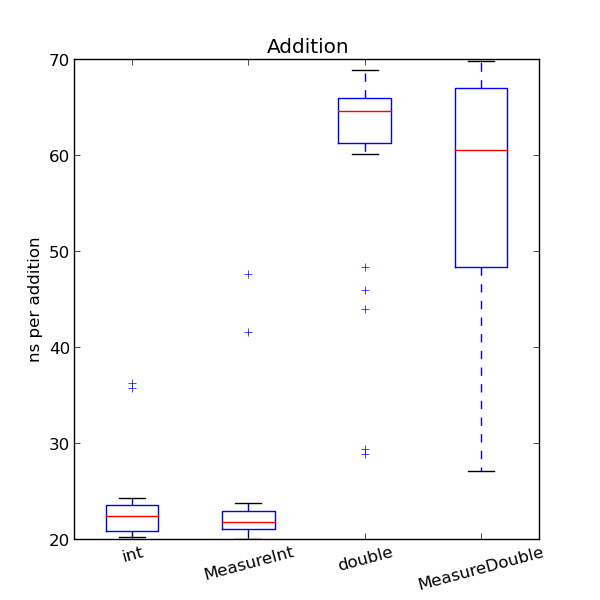
\includegraphics[width=0.49\textwidth]{boxplot_add.png}
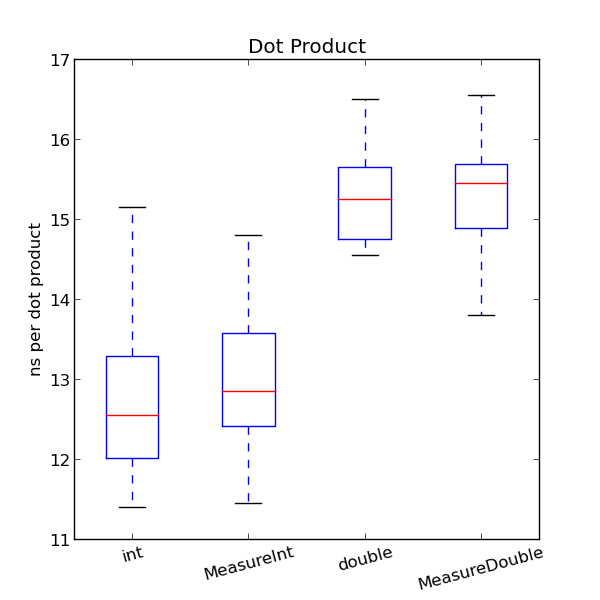
\includegraphics[width=0.49\textwidth]{boxplot_mul.png}
\caption{Runtime for addition and dot product, measured with the methodology described in Chapter \ref{cha:bench}. There is no significant difference between primitives and Measures, although there is of course some variability due to garbage collection.}
\label{fig:rome}
\end{figure*}




\chapter{Future Work}
\label{cha:future}

Two problems remain to be solved that would surpass the scope of this project and are therefore only described here, without offering a full solution. Nevertheless they should be kept in mind when using this Units of Measure library to avoid any potential problems.

\section{Generics}

First, currently it is awkward to combine generics with Measures, as the underlying macros rely on knowing the actual type parameter to perform the correct transformations. A solution to this problem is not easy - either C++ style templates have to be emulated to generate different code for different type parameters, or the unit calculation has to be moved into a compiler plugin.

As a workaround, generic functions can be implemented as macros themselves. Thanks to quasiquoting, this is not too difficult, but care needs to be taken to properly precompute any arguments. Otherwise, performance could drop or a user could run into unexpected side effects (multiple evaluation!). For an example of such an implementation, see Figure \ref{code:scala_generic}.

To further streamline this process, a helper macro could be created. This macro would parse a expression passed in by the user, properly precompute all all values that are used and then emit the correct generic code.

\begin{figure}
\begin{minted}{scala}
/* normal (non-generic) Vector */
case class Vector2(val x: Int, val y: Int) {
  def +(that: Vector2) = Vector2(this.x + that.x, this.y + that.y)
}

/* generic Vector, optimized for Measures based on int */

/* the type bound here is very important, otherwise the value class  *
 * will be boxed (ie T is assumed to be an object), and performance  *
 * is abysmal. check it with 'javap Vector4G' to see the byte code   */
case class Vector2G[T <: MeasureInt[_]](val x: T, val y: T) {
  def +(that: Vector2G[T]) = macro VectorImpl.plus_impl[T]
}

object VectorImpl {
  def plus_impl[T <: MeasureInt[_]](c: Context)
      (that: c.Expr[Vector2G[T]]): c.Expr[Any] = {
    import c.universe._
    val comp = new Precomputer[c.type](c)
    val (aID, bID) = (comp.compute(c.prefix.tree), comp.compute(that.tree))
    val stats = q"Vector2G($aID.x + $bID.x, $aID.y + $bID.y)"
    c.Expr(Block(comp.evals.toList, stats))
  }
}
\end{minted}
\caption{Two different implementations for a 2D Vector. The first is specialized for int, the second uses Generics to accept all Measures that are based on int.}
\label{code:scala_generic}
\end{figure}

\section{Value Classes}
Second, as mentioned in Section \ref{sec:limitiations}, Value classes currently experience degraded performance if used in arrays. This might be fixed in the next version of Scala, offering increased performance with a simple recompilation. Otherwise, a custom array wrapper that stores value classes as raw primitives by manually unwrapping them could solve this problem too. Even without a workaround, this problem is not too serious: performance only drops by about 40\% compared to raw primitives.


\singlespacing
\bibliographystyle{dinat}
\bibliography{thesis}{}
\addcontentsline{toc}{chapter}{A \;References}



\end{document}
